\documentclass[titlepage,10pt]{article}
\usepackage{textcomp}
\usepackage{latexsym}
\usepackage{graphicx}
\usepackage{amsmath}
\usepackage{moreverb} 
\usepackage{pdflscape}
%\usepackage[hmargin=3cm,vmargin=3.5cm]{geometry}


\def\urltilda{\kern -.15em\lower .7ex\hbox{\~{}}\kern .04em}


\begin{document}
\title{
Scaled SWIFT \\
Research Proposal
}

\author{Zouhair Mahboubi}

\date{March $18^{th}$, 2010\\ Stanford University}

\maketitle
\newpage

\abstract
This paper is meant to be a quick overview of the research potential of building a scaled SWIFT model. The goal of the research is to understand effects of scaling on the aerodynamic performance and dynamic response of sub-scale models. We hope to eventually establish a theory and framework to compensate for these effects, in order to be able to better predict in the future for which maneuvers the performance and dynamic parameters obtained from the sub-scale are representative of the full-scale. \\

In the paper, we motivate our choice of the SWIFT as a platform and highlight the potential of collaboration with NASA Ames. We then present some preliminary results of weight, power and price estimation as well as aerodynamic performance for 3 different scales (1/2, 1/3 and 1/4) 

\newpage
\section{Introduction}
The SWIFT is a foot-launched hang-glider with performance similar to a sailplane. The plane has been flown for many years and won numerous competitions. It has also been converted to a powered plane in a pusher-prop configuration. Recently, NASA Ames Research Center (ARC) purchased one of these planes and is planning on converting the airplane into an electrically powered Unmanned Aerial Vehicle (UAV) that would be capable of serving as a technology demonstrator.\\
Our goal is to develop one or two sub-scale models of the SWIFT which can be used as a platform for research in both controls and applied aerodynamics. We intend to coordinate our efforts with the on-going research on the full-scale aircraft, in the hope that data, algorithms, models, etc. can be shared and used on both vehicles.

\section{Motivation}
\subsection{the SWIFT as a platform}
Generally speaking, the weight of a scale-model is proportional to the cube of the scale. With a smaller weight and surface area, the drag of the model airplane and therefore the propulsive power requirement are significantly smaller. With the lower power requirements and reduced weight, a model plane is safer to operate, and cheaper to construct and maintain. Turn-around time for flight-tests is also quicker given the reduced complexity of flight-logistics: model aircrafts are regulated by the Academy of Model Aeronautics (AMA), whereas UAVs operating in the NAS must follow FAA guidelines and need to obtain a permit.\\

In the short term, a scale-model of the SWIFT could be used by NASA-ARC for testing planned modifications or new control algorithms before implementing them on the full-scale plane. This means the possibility of demonstrating new concepts quicker, safer and cheaper. \\

\enlargethispage{2\baselineskip}
The difficulty is in ensuring that the model will have performance and handling qualities similar to those of the full-scale. In order to do this, the scaling needs to maintain some similitude requirements \cite{Wolowicz} (non-dimensional coefficients describing the aerodynamics and dynamics need to be matched). However, it is usually difficult to have all of them matching. And although the use of scale-models for testing aircraft performance is not a new concept, it is still unclear how much error is introduced by incorrect scaling. For these reasons, the SWIFT is an attractive platform given that we would have access to flight-test data of both the model and scale airplanes, thus allowing us to quantify uncertainties on the estimates of performance and dynamic properties caused by unmatched similitude coefficients. Per example, it would be possible to find out which stability derivatives can be trusted from system identification when Reynolds numbers are not matched. We would then investigate methods to account for the discrepancies.\\

\subsection{Research Applications}
The main goal of this project is to establish a theory and framework which would lead to a better understanding of the effects of scaling on aerodynamic performance and dynamic response. In the process, we plan to come-up with methods that would account for these effects in order to better predict the performance of the full-scale model.\\

But since we will have at our disposal a UAV with a relatively high aerodynamic efficiency, we can use it as a testbed for other on-going projects within the Aircraft Design Group: per example dynamic soaring, or characterization of propeller noise (and how it scales). \\

The SWIFT has a low wing loading, and is likely to benefit from solar power. But it's unclear how the addition of panels to the wing affect the airfoil's performance (changing roughness, turbulence onset, etc.) and how the solar-power can be optimally integrated with battery power. This can be investigated on the sub-scale model, and alongside the other applications, could eventually benefit NASA's full-scale UAV. 

\subsection{Literature review}
As mentioned before, the use of models for testing aircraft concepts is not new. NASA itself has a history of using unmanned sub-scale models such as the X-38 Crew Return Vehicle, or the more recent X-48 Blended-Wing-Body demonstrator. But generally speaking, the trend is to construct a scaled model to demonstrate a new technology, before the full-scale airplane is built. One can imagine that at the prototype stage, much of the design is not yet frozen and the full-scale is likely to be different from the sub-scale, thus making it hard to compare flight-test results between the model and the full-scale.\\

A notable exception is NASA's AirSTAR program in which a 5.5\% dynamically scaled version of a B757 was built. The focus of the program however is on 'Integrated Resilient Aircraft Control' which would help prevent loss-of-control accidents. As mentioned in \cite{Airstar} "AirSTAR testbed will be used for [experiments] such as loss-of-control flight due to high angles-of-attack and sideslip, [where] the flow around the aircraft becomes separated and fluid effects associated with Reynolds number scaling may be minimized. For more benign flight conditions, Reynolds number effects can be significant and the aerodynamics of the model would not be representative of the full scale aircraft for certain maneuvers."\\

Our goal is different in that we want to actually understand how significant these effects can be, in order to be able to better predict in the future for which maneuvers the performance and dynamic parameters are representative.

\section{Methodology}
\subsection{Initial Sizing}
\label{sec:initialsizing}
We plan to use traditional methods for the construction (i.e. foam-core and balsa wood mostly) and rely on off-the-shelf RC hobbyist parts and materials to keep the cost down. Initial weight and price estimates (alongside some assumptions) are summarized in Table \ref{tab:scales} and figure \ref{fig:scales}. The assumptions and approach used to come up with weight, power and price estimates are outlined in appendix \ref{app:excel} and included as comments in the spreadsheet. \\

\begin{table}[h]
\begin{center}
\begin{tabular}{|c|c|c|c|c|}
\hline
Scale $\lambda$	& 1 & 1/2 & 1/3 & 1/4 \\ \hline
Span (m)	& 13& 6.5 & 4.3 & 3.25\\ 
Mass (kg)	& 150& 18.7 & 5.6   & 2.3 \\
Cruise(m/s)	& 17 & 12 & 9.8   & 8.5 \\
$Re_{avg}$  	& 1,150,000 & 400,000 & 220,000 & 140,000 \\
Froude		& 29.5 & 29.5 & 29.5 & 29.5 \\
Motor Power (W) & 11000 & 1360 & 400 & 160 \\
Endurance (min) & 180  & 100 & 65 & 20 \\
Price $\approx$ (\$) & $>$40000 & 6500 & 4000 & 3200 \\
\hline
\end{tabular}
\caption{Scale Comparison}
\label{tab:scales}
\end{center}
\end{table}

In all cases, the spreadsheet gives a way of computing the minimum weight of the vehicle, we then adjust the payload (here assumed to be completely batteries) carried by the airplane in order to match the Froude number and non-dimensional mass. Based on this initial sizing, a 1/4 scale model would be straight-forward to construct and operate, but difficult to match these coefficients and still have a high endurance (some of the assumptions for fixed weight components also had to be relaxed since otherwise the Froude number would be too hight). A 1/3 scale-model would be useful while remaining manageable, while a 1/2 scale is doable with off-the-shelf RC hobbyist parts but the logistics for operation are somewhat harder.  We leave the decision of which scale should be pursued to after the discussion about Reynolds numbers and moments of inertia. The details of the computation steps are given as comments in the spreadsheet.\\

The price estimates for the models are for the material and components and include about \$2000 for the autopilot and sensors. Figure \ref{fig:scales} plots the ratios of these estimates relative to the full-scale airplane. Since matching the Froude number and non-dimensional mass puts constraints on the weight and flight speed, the mass and power turn out to be cubic in the scale $\lambda$ while the Reynolds number varies with $\lambda^{1.5}$

\begin{figure}[h]
\begin{center}
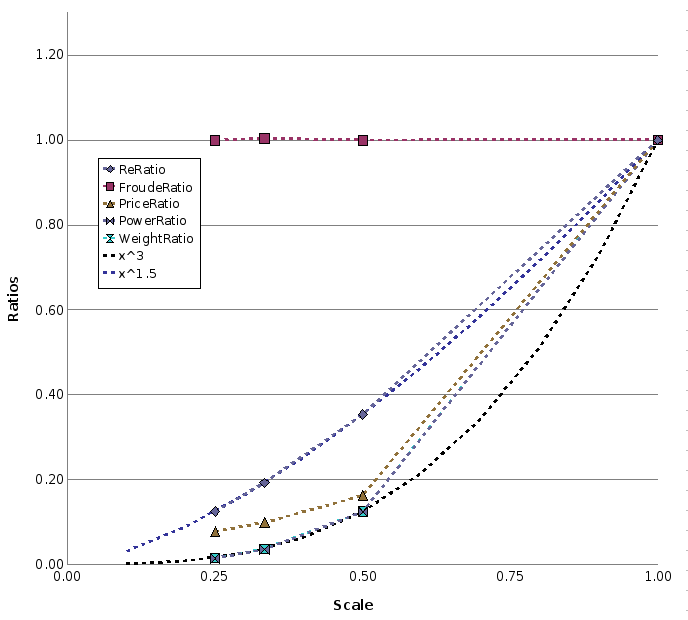
\includegraphics[width=140mm]{scale-graph.png}
\end{center}
\caption{Similitude Parameters versus Scale}
\label{fig:scales}
\end{figure}

\clearpage


\subsection{Autopilot and Sensors}
We are likely to fly the airplane with a remote controlled radio before moving to an autonomous vehicle. But even in the initial phases, having an autopilot which serves as an 'avionics' unit to log inputs and responses is necessary.\\

Since our goal is not particularly to develop a new autopilot, an off-the-shelf one would be preferable. We require a board that has enough PPM channels to command at least 8 servos and one Electronic-Speed-Controller, 3 serial ports (radio, GPS and IMU) and 5 to 8 A2D converters for the alpha-beta veins, pressure sensors, etc. Moreover, we would like to have fairly decent onboard computing power in the event we decide to use more advanced control algorithms or carry scientific payload. Unfortunately, most commercially available autopilots are closed-source and tend to be cost-prohibitive, which forces us to turn to the DIY scene. However, even the most mature DIY systems have limited processing power, serial and I/O ports.\\

For these reasons, we are considering to use the open-source \textit{Paparazzi} software in conjunction with a \textit{Roboard} hardware. We chose this architecture because the \textit{Roboard} hardware satisfies our requirements. A similar approach has been carried-out by other groups, and the \textit{Paparazzi} has a good track record of being used on different hardware architectures (ranging from Gumstix to x86 computers\footnote{A recent effort by students from Rutgers University has successfully ported the paparazzi to a beagleboard running linux http://moreproductive.org/autopilot/})\\

The reason we want to use the \textit{Paparazzi} is that after having worked with it for 6 months, we think that some of its functionalities such as in-flight tuning make flight-testing easier. Moreover, its support for both state-machine, 6DOF and HITL simulations help reduce development and testing time. The point is that while we could develop our own autopilot from scratch, we can avoid 'yet-another-autopilot' by leveraging the \textit{Roboard} and \textit{Paparazzi} capabilities and online communities.\\

\begin{figure}[h]
\begin{center}

\includegraphics[width = 30mm] {paparazzi.png}
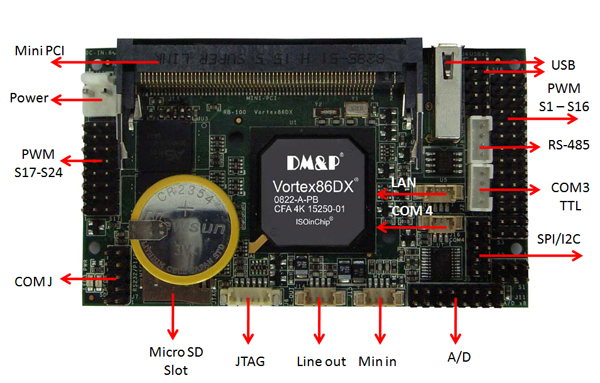
\includegraphics[width = 30mm] {Roboard.png}
\caption{Paparazzi Software and Roboard Hardware}
\end{center}
\end{figure}

\newpage
\subsection{Issues with small Reynolds numbers}
A 1/4 scale has the advantage of being roughly the size of most RC models, which means that flying it would be relatively easy. The problem however, is that at this scale Reynolds numbers are so small that the airfoil characteristics are likely to suffer, especially at high lift-coefficients. In order to analyze the effect of this, we have used Xfoil to generate section data at different Reynolds numbers. The analysis is viscous and assumes a trip location at 20\%. We focus on the conditions on the inboard sections since the wing has about 10 degrees of washout, so although the Reynolds number is smaller at the tip, the angle of attack there is smaller and tip stall should not be an issue. That being said, rather than keeping the Reynolds number fixed at all angle of attacks, we hold $Re\sqrt{Cl}$ fixed since we expect that at higher lift coefficients the wing is going to be flying slower and thus at a reduced Reynolds number (an analysis with fixed Reynolds number was also carried out, the results are not presented since the overall conclusions are the same).\\

Figure \ref{fig:xfoil1} shows the 2D sectional lift, drag and moments versus angle of attack at the 4 Reynolds numbers (Re) of interest. As expected, at lower Re the sections have higher drag and before stall the lift is linear in angle of attack. The maximum lift coefficient are significantly lower for 1/4 and 1/3 cases. This is also expected, but the surprising result is that for the 1/2 scale case, the stall occurs at roughly the same position thus allowing the section to reach the same $Cl_{max}$. This seems to be counter-intuitive since lower Re are usually associated with an earlier onset of separation.\\

One explanation for this might be that near high angle of attacks, the higher Re airfoil transitions to turbulent flow before reaching 20\% of the chord, while the smaller Re remains laminar. So for a given pressure gradient, the higher Re separates earlier because the boundary layer is not as healthy as the smaller Re which had a laminar rooftop. To test this hypothesis, we looked at the case where the flow is tripped at 1\%. The resulting lift curves are presented in figure \ref{fig:xfoilstall} where we can clearly see that stall occurs earlier in the lower Re case. Another thing we notice is that the maximum lift-coefficient is also smaller. This is because without laminar rooftop, the flow is less able to remain attached against the high pressure gradients associated with the higher lift.\\

Finally, we also looked at the airfoil's performance with a deflected flap. The results are shown in figure \ref{fig:xfoilflap}. We again notice that for the 1/3 and 1/4 case the onset of stall is significantly earlier than for the 1/2 and full-scale. This alongside the previous results seems to indicate that it would be possible to build a 1/2 scale model using the same airfoil as the full-scale, while we would need to redesign the airfoil for the 1/3 or 1/4 scale models.


\begin{landscape}
	\begin{figure}
	\begin{center}
	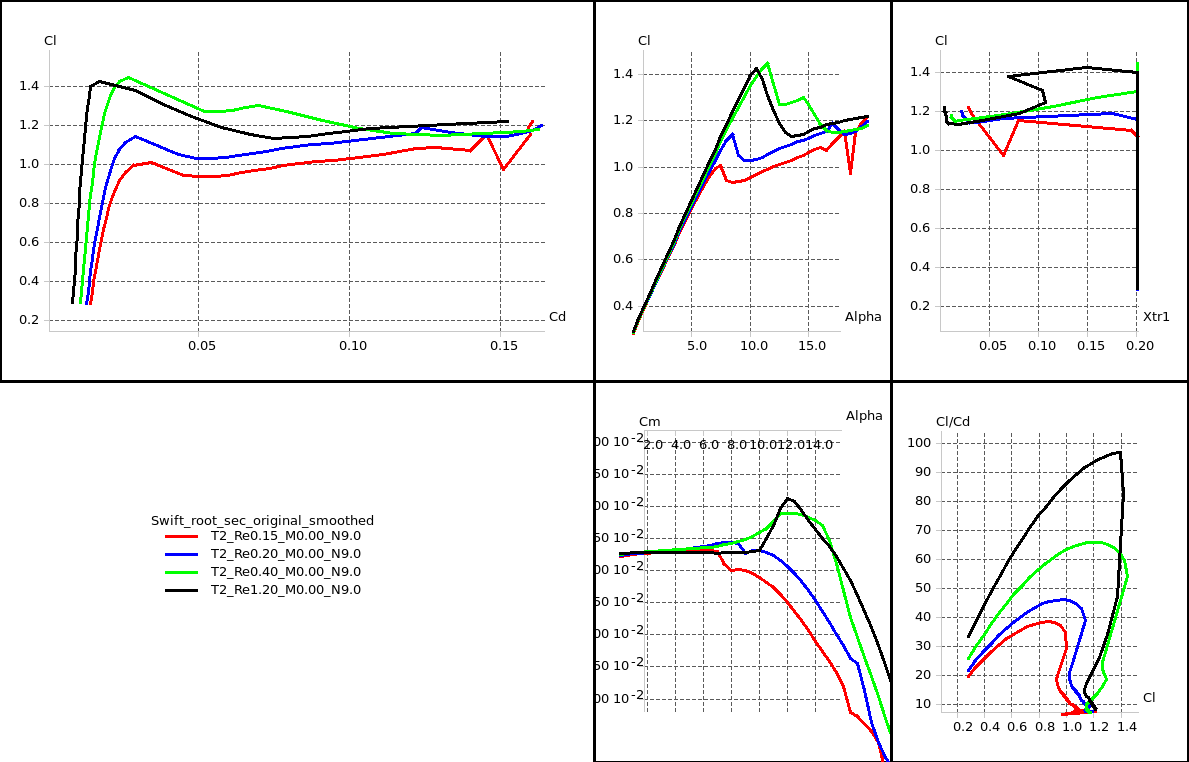
\includegraphics[width=220mm]{xfoil_T2_analysis.png}
	\end{center}
	\caption{Cl, Cd and Cm for Swift airfoil section at different Reynolds numbers}
	\label{fig:xfoil1}
	\end{figure}
\end{landscape}

\begin{landscape}
	\begin{figure}
	\begin{center}
	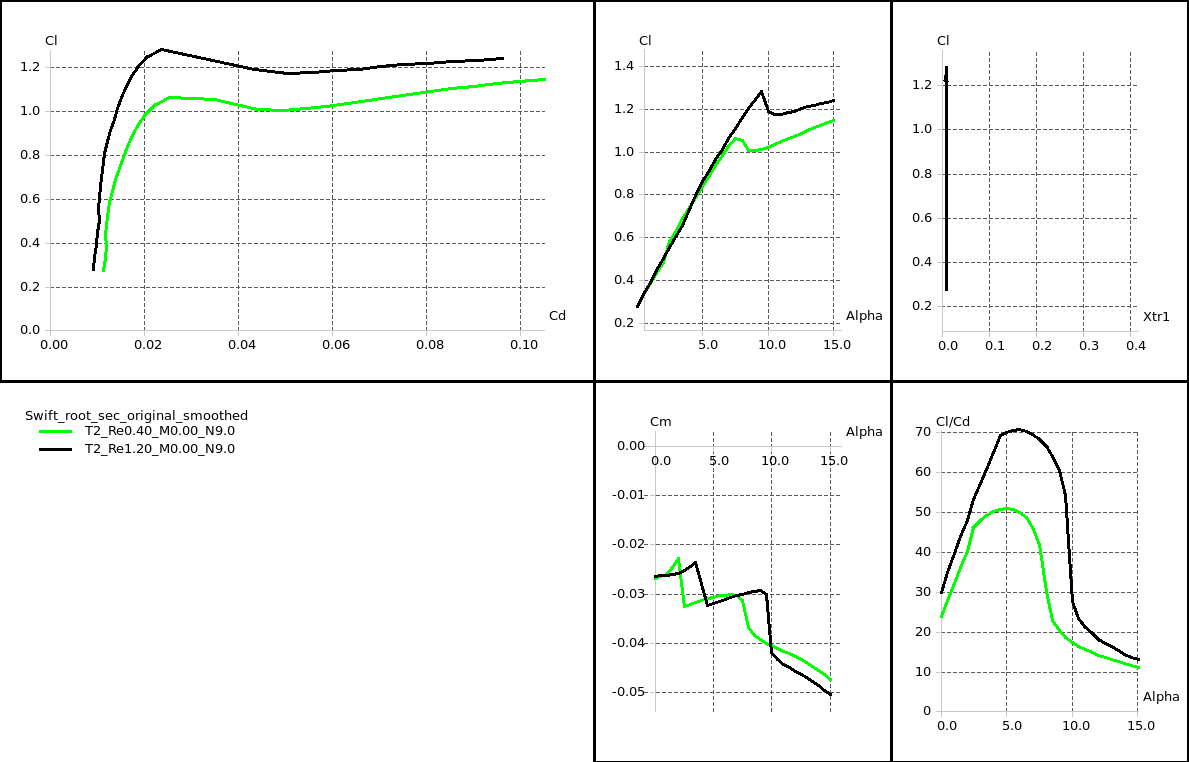
\includegraphics[width=220mm]{xfoil_T2_analysis_stall.png}
	\end{center}
	\caption{Cl, Cd and Cm for Swift airfoil section with trip location at 1\%}
	\label{fig:xfoilstall}
	\end{figure}
\end{landscape}

\begin{landscape}
	\begin{figure}
	\begin{center}
	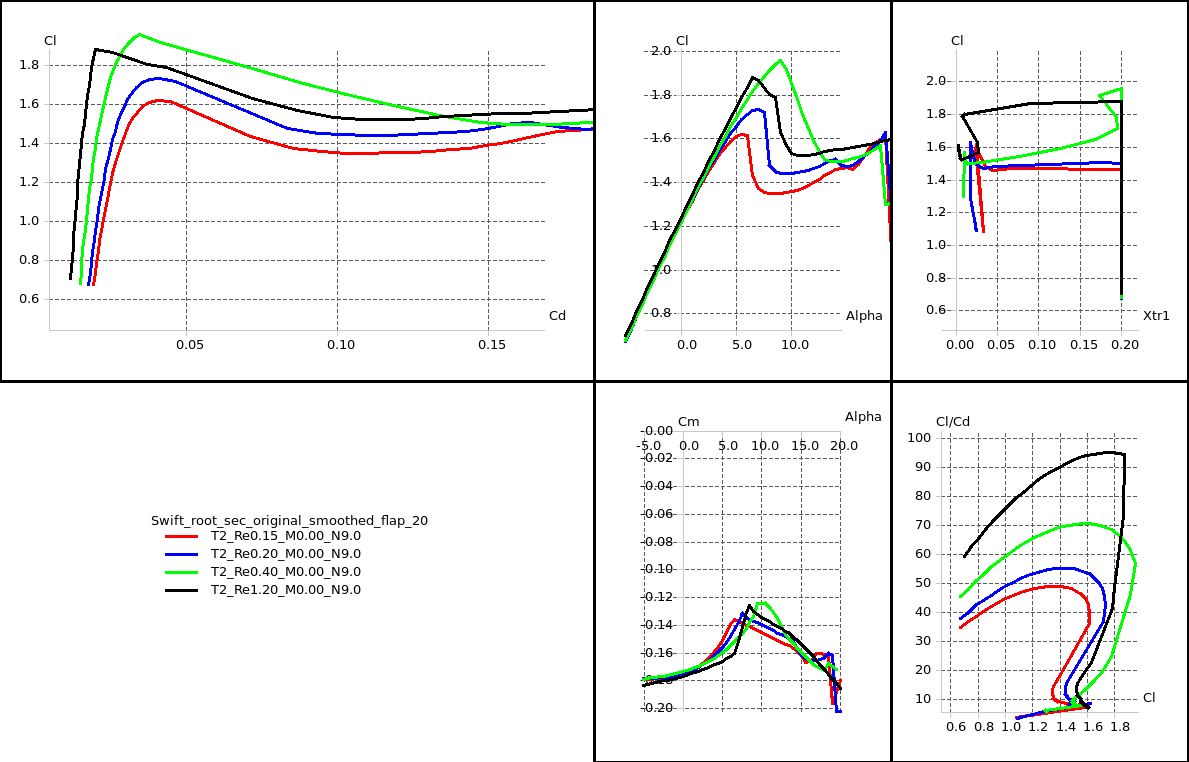
\includegraphics[width=220mm]{xfoil_T2_analysis_flap20.png}
	\end{center}
	\caption{Cl, Cd and Cm for Swift airfoil section with $20^o$ flap at different Reynolds numbers}
	\label{fig:xfoilflap}
	\end{figure}
\end{landscape}



\subsubsection{Tripping the Boundary Layer}
So far we have assumed that we are able to cause the flow to transition from laminar to turbulent at 20\% of the chord regardless of the Reynolds number. In order to accomplish that, we are going to need some sort of turbulator device. A good discussion on trip strips is available in \cite{WindTunnel}, and a simple method by Braslow \cite{Gritheight} based on the Reynolds number per distance (R) can be used to compute the minimum grit height $h \approx 600/R$. However, while strips of grit are the traditional method for wind tunnel testing, a two-dimensional tape or a three-dimensional pinked tape (aka zig-zag tape) might be more suited for us since grit tends to break away from the adhesive after repetitive testing. It is unclear whether the method of determining grit height can be applied for tape height. An alternative approach is outlined by Martin Hepperle \cite{Hepperle} for the sizing of strip of tape turbulators and is summarized by figure \ref{fig:turbulator}

	\begin{figure}[h]
	\begin{center}
	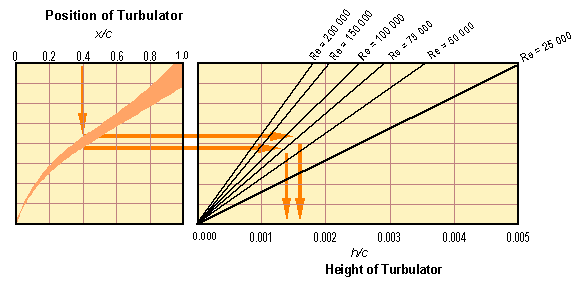
\includegraphics[width=100mm]{turbulator_height.png}
	\end{center}
	\caption{Turbulator height selection chart (from \cite{Hepperle})}
	\label{fig:turbulator}
	\end{figure}

For all scales, Hepperle's method requires us to use $h/c$ in the range of .0005 to .001, while Braslow's method leads to $h/c$ about three times larger in the range of .0015 to .004. We should keep in mind that the two methods assume different turbulator materials, so it is quite possible that the tape height does need to be different from the grit height.\\

Considering that tripping the flow is crucial for this airfoil design (with free transition, the $Cl_{max}$ is greatly affected even for the full-scale airfoil), this is a detail that needs to be figured out. We are currently in touch with some of the people at the Fluid Mechanics lab at NASA Ames in an attempt to answer this question. That being said, if we do use tape we always have the possibility of increasing the thickness gradually by layering multiple levels until a satisfactory performance is achieved.

\newpage
\subsubsection{Extension to 3D}
In order to properly account for all 3D effects, a full RANS solution would be necessary. However, we can try to obtain some rough estimates of the full 3D wing performance by using a vortex-lattice code (XFLR5 \cite{XFLR}, figure \ref{fig:xflr3D}) to generate angle-of-attack sweeps for the different scales and masses. This code assumes that each section of the wing behaves as in 2D flow, and interpolates the drag polars from xfoil using the section lift coefficient computed from a VLM method. The lift was constrained to match the weight so that different velocities and Reynolds numbers are used. The curves are truncated after one of the wing's sections stalls since the data can no longer be interpolated. \\

The results of using the same 15\% thick sections at different scales are shown in figure \ref{fig:tc15} (wing is at an incidence of $10^o$). We notice that the full-scale achieves a maximum ${C_L}$ of 1.2, while the 1/2 reaches ${C_L}_{max}\approx1.05$ and the 1/3 and 1/4 are way past stall by 0.7. For the 1/3 and 1/4 scale the sharp decrease of the lift-to-drag ratio ${C_L}/{C_D}$ begins at around ${C_L}=0.6$ indicating that portions of the wing have already started to stall (this could be explained by the inboard sections stalling, see discussion in appendix \ref{app:stalled}). This is clearly unacceptable since we expect to cruise at ${C_L}=0.7$ (optimal L/D)\\

In all cases, the pitching moment coefficient ${C_m}$ and pitching moment derivative \footnote{CG position relative to the leading edge is at the same fraction of the MAC for all scales} ${C_m}_{\alpha}$ are hardly changed as predicted by thin airfoil theory \footnote{Small changes in Cm are due to difference in Boundary Layer thickness at different Re}. It's worth pointing out that the drag coefficient even for the 1/2 scale model is higher since airfoils have generally lower L/D at lower Reynolds numbers.\\

So although the 1/2 scale is not able to achieve the same maximum lift coefficient as the full-scale, it comes to within 12\% of it. So if we are willing to accept this reduction in the flight envelope, a 1/2 scale model would realizable without needing to redesign the 2D section airfoil. Otherwise, it is worth pointing out that the difficulty seems to be around Re of 300,000 (for Reynolds numbers above that, the maximum lift coefficient is unaffected. So It might be worth looking into small modifications of the airfoil to push this 'critical' to a lower value).\\

As for the 1/3 and 1/4 scales, this method just re-iterates the conclusion we reached from the 2D analysis, that is the airfoil is going to perform poorly at those low Reynolds numbers.



\begin{landscape}
	\begin{figure}
	\begin{center}
	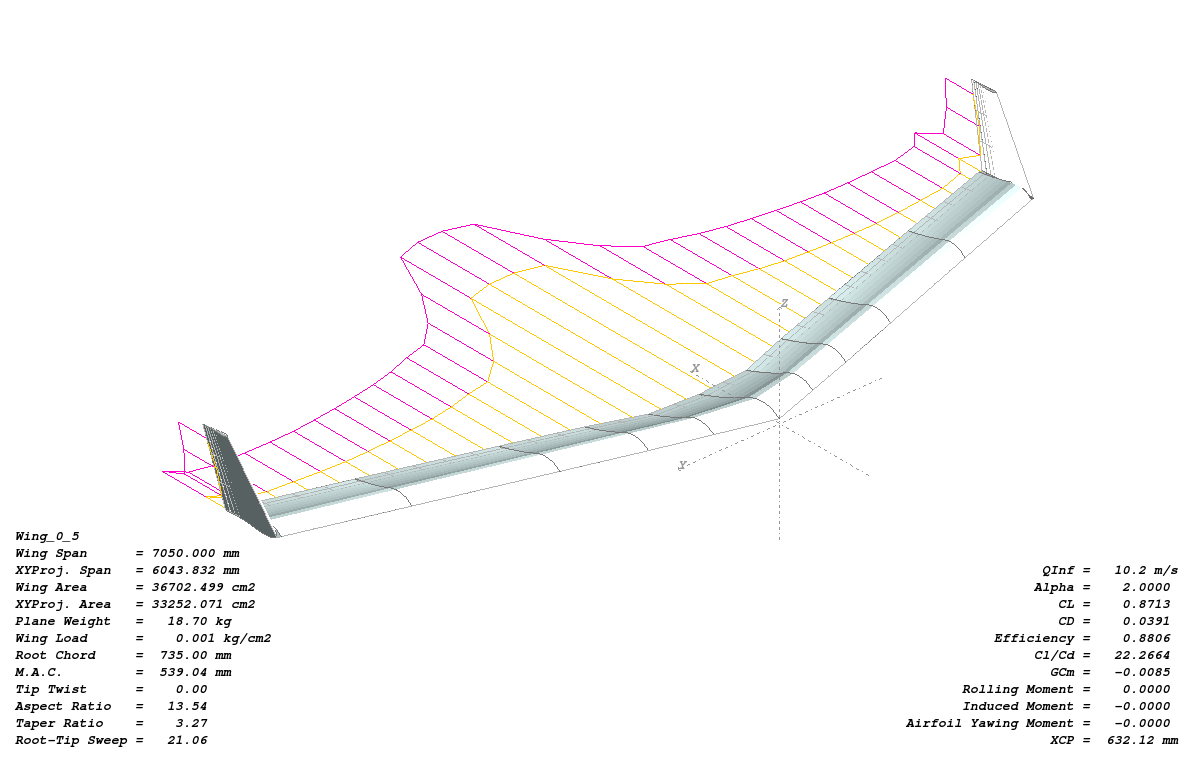
\includegraphics[width=220mm]{XFLR_3Dview_simple.png}
	\end{center}
	\caption{3D Geometry of the 1/2 scale model at AoA $2^o$}
	\label{fig:xflr3D}
	\end{figure}
\end{landscape}

\begin{landscape}
	\begin{figure}
	\begin{center}
	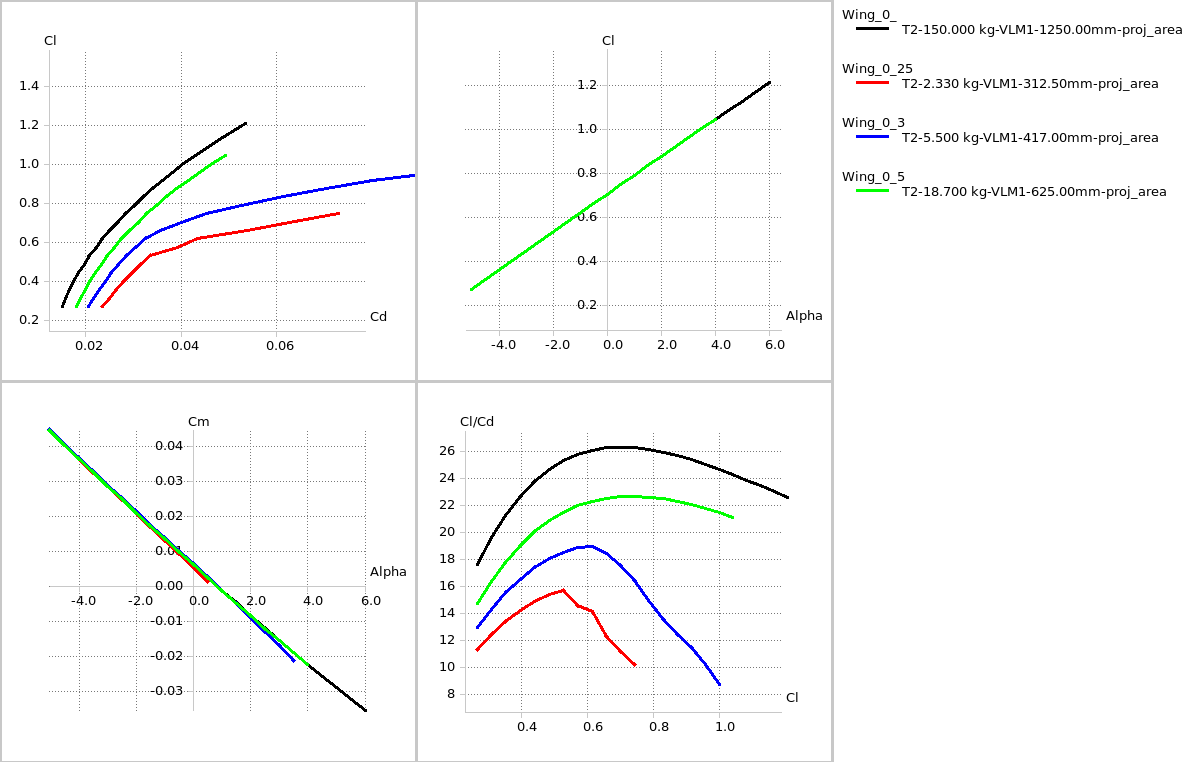
\includegraphics[width=220mm]{scale_original_airfoil_15.png}
	\end{center}
	\caption{15\% thick Airfoils for all scales}
	\label{fig:tc15}
	\end{figure}
\end{landscape}


\clearpage
\newpage

\subsection{Scaling and Measurements of Moments of Inertia}
One part that we have not addressed in the scaling is the difference in mass moments of inertia. While we don't expect them to have an effect on the stability derivatives and non-dimensional coefficients, they clearly will affect the longitudinal and lateral mode frequencies of the vehicle. So if the actual handling response is of interest, it is therefore necessary to properly scale the moments of inertia in order to match the frequency response of the vehicle; on the other hand, if only the stability derivatives and non-dimensional coefficients are of interest, the scaling of the moments of inertia is of little importance as long as the vehicle remains stable.\\

That being said, sometimes a lot of effort goes into properly scaling the moments of inertia of a model. Per example, this has been done with the X-48B in order for the full-scale dynamic response to be accurately estimated from the sub-scale flight characteristics. An interesting question that can be investigated as part of this project is whether it's possible to synthesize an "co-pilot controller" that modifies the dynamics of the sub-scale model in order to match the frequency response of the full-scale vehicle. Moreover in order to estimate the aerodynamic coefficients from flight-tests, it is usually necessary to have good estimates of the mass and inertia properties of the airplane. Indeed, one of the conclusions of the preliminary flight test results of the X-48B is that there is a trade-off between estimating the kinematics and aerodynamics of the aircraft, and that \textit{"the parameter estimation [is] only as accurate as the aircraft inertia [estimates]}" \cite{X48B}.\\

While it is possible to measure inertias for a small sub-scale aircraft through a series of single degree-of-freedom oscillations, it can be a more challenging task for a larger aircraft where it's unsafe to hang the plane in all degrees, and therefore a meticulous component build-up is required. We believe that it might be possible to estimate moments of inertia from flight-tests as well. The idea would be to carry-out different flights where the weight and mass distribution of the airplane are carefully changed. Because the aerodynamic performance would remain unchanged (stability derivatives are only a function of the planform), it would be possible to estimate the inertia properties more accurately. We plan to investigate this technique on the small-scale plane and hopefully apply it to the full-scale one.\\

When scaling moments of inertia, there are two quantities of interest. The magnitude of the moments relative to each other, and their magnitude relative to the 'displaced air' $I/(\rho c^5)$. As far as the Swift is concerned,  we currently only have estimates from CAD models of the wing geometry and the major components estimated as point masses. In the CAD model we assumed a constant skin thickness to chord ratio and homogeneous material for the entire wing.\\
\newpage

We did the same thing with the scaled versions as well using both full and hollow wing cores (we only considered the wing's contribution since even for the full scale, it is mostly the Iyy and Ixz terms that are affected by the other components). But it turned out that the thickness of the skin is only important in determining the weight of wing (a full core foam wing will weight much more than a hollow core), but for a given weight the moments of inertia are only a strong function of planform (the actual thickness will modify Iyy, but not as much as say the engine and battery placement will). We also used the XFLR5 software to estimate the moments of inertia in order to double check our estimates. For a given wing weight and vehicle scale, the two methods agreed well apart from the Iyy term which was slightly larger in XFLR5 as expected since it does not support hollow wings.\\
		
\begin{table}[h]
\begin{center}
\begin{tabular}{|l|c c c|}
\hline
Full scale & X & Y & Z \\
\hline
 & 517     &-0.14	&7.05 \\
 &	&38	&-0.3 \\
 &	&	&542 \\
\hline
Half scale & & &\\
\hline		
 $\Delta I_{xx} = -10\%$  & 468	&0.4	&-0.7 \\
 &	&15	&0.00 \\
 &	&	&482 \\
\hline
Third scale & & &\\
\hline		
 $\Delta I_{xx} = -16\%$  & 446	&0.1	&-0.5 \\
 &	&14	&0.00 \\
 &	&	&450 \\
\hline
Quarter scale & & & \\
\hline		
 $\Delta I_{xx} = -19\%$ & 434	&0.1	&-0.5 \\
 &	&14	&0.00 \\
 &	& 	&449 \\
\hline
\end{tabular}
\caption{Normalized Moments of Inertia $I/(\rho c^5)$}
\label{tab:inertia}
\end{center}
\end{table}

Table \ref{tab:inertia} summarizes the moments of inertia of the wing as estimated by the CAD model normalized by the fifth power of the mean aerodynamic center. The weights of the wings were the ones computed within the spreadsheet. These results assume a hollow foam core. Indeed, we quickly realized that when using a full core, the normalized moments of inertia end up being much larger for the scaled models. This is mainly because as mentioned above the wing ends up being too heavy. This means that it would be impossible to scale the moments of inertia if a full core foam wing is used in the construction.\\
\newpage

So in a sense, matching the non-dimensional moments of inertia imposes a constraint on the weight of the wing which needs to vary with the cube of the scale $\lambda$. This is because under the assumption of a homogeneous material, the mass moment inertia will scale linearly with the average material density and the area moment. The former depends on the weight of the wing and the latter scales like $\lambda^2$. Because the non-dimensional moments of inertia are normalized by $c^5$, in order for them to remain constant, the wing weight must vary with $\lambda^3$. \\

This means then that the weight we estimated for the 1/2 wing is 10\% too small. Considering that additional weight was required to match the other non-dimensional values, this should not be a problem. We can always make the spar thicker, and thus the wing stronger and remove some of the batteries in order to maintain the same total weight. We should also keep in mind that 10\% is probably within our estimate accuracy, and that these estimates don't include the effect of placing the servos on the wing.\\

 The same thing can be said for the 1/3 scale, but the 1/4 scale is more problematic. Indeed, matching the moments of inertia requires a heavier wing, but as mentioned in previous sections matching the mass ratio limits the endurance and weight of the other components. Of course this does not mean that it would be impossible to match the moments of inertia. Since the wing does not necessarily need to be homogeneous, it is possible to add point masses at some spanwise location to match the moments of inertia, thus keeping the wing's weight small enough to match the mass ratio while still having a reasonable endurance.\\

Finally, we point out that although the $Iyy$ and $Ixz$ terms seem to be significantly different, they are mostly affected by the engine, batteries and avionics placement. So it is normal that our estimates of these moments are much smaller for the scaled vehicles since we only considered the wing in our analysis of the scaled vehicles.


\newpage
\section{Conclusions}
The goal of this report was to identify potential research topics that can be pursued were we to build a sub-scale of the Swift. On the short term, a sub-scale vehicle would benefit NASA's full-scale UAV by providing a test-bed. On the long term, we would like to establish a theory and framework which would lead to a better understanding of effects of scaling on aerodynamic performance and dynamic response. There is of course also potential to use the vehicle by other Stanford affiliates as a testbed for new control algorithms, propeller noise characterization, electric propulsion system integration, etc. \\

Using a component buildup approach we estimated the total weight of the vehicle for different scales. In the process, we made sure that the dynamic similitude parameters (Froude and mass ratio) were matched. We found that all three scales considered (1/2, 1/3 and 1/4) would be feasible using mostly off-the-shelf RC hobby parts. However, we identified that the smaller Reynolds numbers would be an issue, and investigated which scales would suffer the most from this. We found that the 1/2 scale would be able to use the same airfoil as the full-scale, while the 1/3 and 1/4 scale would need a redesigned airfoil. \\

We have also compared the non-dimensional moments of inertia and showed that for the 1/2 and 1/3 scale, matching them should be possible as long as the wing is constructed such that its weight is proportional to the cube of the scale. This is straightforward since at those scales additional ballast weight in the form of batteries or thicker spars is necessary. For the 1/4 scale, the overall vehicle weight is constrained by the other similitude parameters, which ends up reducing the total vehicle indurance and potentially requiring point masses along the span to properly match the inertias.\\

While a 1/4 scale is the easiest to manufacture and operate, our analysis seems to indicate that in order to match all the dynamic and performance coefficients, the airfoil would need to be redesigned, the vehicle's endurance would be limited and matching the moments of inertia might to be more difficult. The 1/3 scale vehicle would also require a redesigned airfoil, but it would not suffer from a limited endurance like the 1/4 scale. As for the 1/2 scale, it can use the same airfoil as the full-scale and still allow us to match most of the flight-envelope all while having a significant endurance allowing it to be potentially used in other applications. But it is likely going to take longer to manufacture, and be more complicated in terms of operation.\\

\enlargethispage{4 \baselineskip}
In conclusion, we do not think that building a 1/4 scale would be worthwhile. We can make a case for the 1/3 scale, especially that investigating the redesign of the airfoil in order to match the full-scale performance might be interesting. However, a 1/2 scale Swift would provide us with a vehicle that would be capable of matching the characteristics of the full-scale Swift while still being 8 times lighter, requiring 1/8th of the power and using affordable off-the-shelf parts. Sure at that scale the airplane is going to have to be flown in restricted airspace, but at least it is likely to be classified under the Class-I low-risk category as opposed to medium or high risk like the full-scale.


\newpage
\subsection{Time-line and Future work ... }
\enlargethispage{3 \baselineskip}
This is a very rough time-line... \\
Design in Winter-Spring 2010: Settle on a scale, redesign airfoil if necessary, measure inertias on full-scale Swift, pick out components/sensors/etc, make drawings for subsystems, develop autopilot/FBW system, carry out more detailed analysis of the structure (especially if building 1/2 scale).\\
Begin Construction in Summer 2010 ... Depending on scale, Initial flight-testing in Fall or Winter of next year.\\


\newpage
\appendix
\section{Weight, Power and Price Estimates}
\label{app:excel}
The results presented in section \ref{sec:initialsizing} were obtained from calculations using an Excel spreadsheet. In doing so, we used some assumptions to simplify the analysis. The spreadsheet is included with the report and has comments which summarize the content of this section.\\

The spreadsheet also reports some of the scaling factors, it is then possible to vary the payload (or the endurance, i.e. number of batteries) to try to match these coefficients. Since the design of the airplane is technically already fixed, this greatly simplifies the weight estimation process. We break down the weight into four major subcomponents:

\subsection{Wing Weight}
\subsubsection{Foam core weight}
The weight of the foam core is computed using the wing volume which is obtained from a CAD model of the Swift. The density of the foam is assumed to vary between 21$kg/m^3$ and 37$kg/m^3$ depending on the scale of the model. The spreadsheet allows using a full-core or hollow-core. Note that the full-core tends to have too high of moments of inertia.

\subsubsection{Skin Weight}
The skin weight is assumed to be proportional to the wetted area of the wing. Once again, this is obtained from a CAD model. The density of the skin is assumed to vary between 0.17$kg/m^2$ and 0.35$kg/m^2$ depending on the scale. In order to account for the weight of the resin, we researched the volume ratio of the fabric and using density of the resin estimated that the density of the matrix soaked in resin is a factor of 1.5 to 2.5 that of the fabric alone. We used an average of 2 in our calculation in the spreadsheet.

\subsubsection{Spar Weight}
We assume that we will be using carbon-fiber spar caps with a constant thickness. The design assumes an elliptical lift load which is integrated to find the maximum bending moment at each cross section along the span. We assume that the spars height is constrained by the width of the airfoil sections, while their width is a fixed percentage (5\%) of the root section chord. The required thickness to carry the bending load is then computed, and the entire volume is integrated to obtain the total mass of the spar. For simplicity, we precompute the percentage of the spar weight for a range of vehicle weights and use that inside the spreadsheet. The matlab routine used for this is included in appendix\ref{app:sparsizing}. 

\subsection{Fuselage Weight}
The fuselage is assumed to be constructed using the same material for the wing skin. The surface area of the fuselage is obtained from the CAD model and is approximatively 1/4th of the wing wetted area.

\subsection{Propulsion System Weight}
\subsubsection{Power Estimation}
In order to estimate the weight of the propulsion system, we need to first estimate the power required by the model plane. We begin by assuming a cruise lift coefficient and a lift-to-drag ratio (this could be estimated from a quadratic drag equation but we would have to assume a zero-lift drag coefficient instead). We also assume a propeller and propulsion efficiencies. We can use $$P_{cruise,req} = D*V_{cruise}/\eta = \frac{W\ V}{\eta \frac{L}{D}}$$ to estimate the required cruise power. However, we need to be able to achieve a minimum climb rate. So we use instead $P_{req} = T*V_{cruise}/\eta$ where T can be obtained from $(T-D)=\gamma*W$ with $\gamma$ being the climb path angle. Using these relations we find that $$P_{climb,req} = \frac{W\ V}{\eta \frac{L}{D}}(1+\gamma \frac{L}{D})$$
The spreadsheet takes a climb rate h as an input and computes $\gamma=h/V$. We estimated the climb rate of the full scale to be $h=4m/s\approx800ft/min$ and used that in our calculations.

\subsubsection{Motor and actuator Weight}
Given the required power from the motor, we can use statistical methods to estimate the weight of the motor. We rely on the data given in the AxiMotors catalog to come up with simple fits. We were conservative in these estimates in order to allow for extra weight due to wires, ESC and propeller. As for the actuators, we were unable to find a simple relation between the torque rating and weight. So instead we assume a fixed weight per actuator with different values for each scale.

\subsubsection{Battery Weight}
The battery weight is computed by determining the required energy to achieve a desired endurance. The endurance can be set in the sheet and is varied in order to match the non-dimensional Froude and mass ratios (basically increasing the payload). We assume that 30\% of the time is spent in climb and the rest in cruise. The battery capacity in mAh is then computed from the voltage (i.e. number of cells). Given the required capacity we can compute the weight by assuming an energy density which is fairly constant over a large range for Lithium Polymer batteries. 


\subsection{Avionics Weight}
We assume this to be a fixed weight which includes the autopilot board, sensors and a 2000mAh LiPo for power. The values assumed for the 1/4 scale are smaller since otherwise it is difficult to match the mass ratio and Froude number while still having a reasonable endurance.


\subsection{Weight Iteration}
The motor weight estimation relies on the required power, which in turn is a function of the total weight. However, we initially don't know the total weight since we only estimate the structural weight. So we need to iterate until we converge to a total weight which accounts for the structural weight and propulsion weight. The same process needs to be carried out for the weight of the spars.

\subsection{Price Estimates}
Most of the price estimates are statistical fits to values quoted by online suppliers. Whenever possible an explanation or link is given in the spreadsheet. It's worth noting that the cost does not include 'tooling' cost as we assume it will be available at the lab.


\newpage	
\section{Stalled Inboard Sections}
\label{app:stalled}
In the analysis due to changes in Reynolds Numbers we have compared maximum lift coefficients and lift-to-drag ratios for the entire wing at different scales. We made the claim that although in some cases the entire wing is able to reach a high-lift coefficient, the sharp decrease of $C_L/C_D$ at lower values of $C_L$ indicate that the wing was partially stalled. The following figure which shows the span-wise distribution of the local drag coefficient $C_d$ of the three different scales at a fixed AoA and $C_L=0.87$. It's normal that $C_d$ increases as we approach the wing root since the local lift coefficient $C_l$ is higher due to the washout (the discontinuity at the tips are due to the winglets). However, it is clear that in the case of the 1/3 scale, there is an abrupt increase in $C_d$ for the inboard sections, indicating that those sections have stalled.

\begin{figure}[h]
\begin{center}
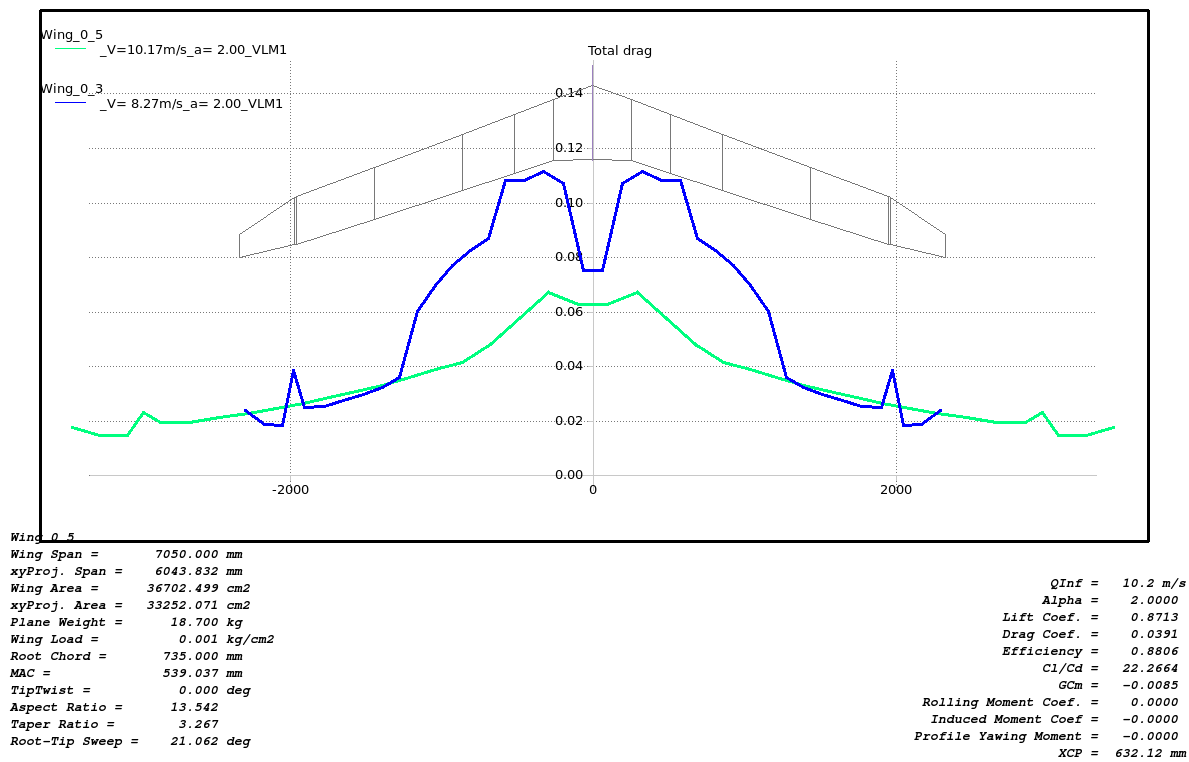
\includegraphics[width=120mm]{XFLR_spandrag_stall.png}
\end{center}
\caption{Spanwise distribution of the local drag coefficient Cd}
\label{fig:tcdrag}
\end{figure}

\clearpage

\newpage
\section{Matlab Routine for Spar Sizing}
\label{app:sparsizing}
\verbatimtabinput[8]{spar_sizing.m}

\newpage
\begin{thebibliography}{9}

\bibitem{Wolowicz}
   Wolowicz, C.H., Bowman, Jr., J.S., and Gilbert, W.P.,
   “Similitude Requirements and Scaling Relationships as Applied to Model Testing”, 
   NASA TP-1435, 1979.

\bibitem{Airstar}
	Thomas L. Jordan, et Al.,
	"AirSTAR: A UAV Platform for Flight Dynamics and Control System Testing"
	NASA Langley Research Center

\bibitem{X48B}
	Brian R Taylor,
	"X-48B Preliminary Flight Test Results".
	Fundamentals Aeronautics Program, Subsonic Fixed Wing Project.
	2009 Annual Meeting

\bibitem{XFLR}
	A. Deperrois,
	"XFLR5 analysis tool for airfoils, wings and planes",
	2009
	Project Page http://xflr5.sourceforge.net/xflr5.htm

\bibitem{Hepperle}
	Martin Hepperle,
	"Turbulators".
	August 2003.
	http://www.mh-aerotools.de/airfoils/turbulat.htm
	[Retrieved March 11th 2010]

\bibitem{WindTunnel}
	William H. Rae, et Al.,
	"Low-Speed Wing Tunnel Testing".
	John Wiley \& Sons, 1984.

\bibitem{Gritheight}
	Albert L. Braslow et Al.,
	"Simplified Method for Determination of Critical Height of Distributed Roughness Particles for Boundary-Layer Transition at Mach Numbers from 0 to 5".
	Langley Aeronautic Laboratory, 1958.
\end{thebibliography}


\end{document}
